\documentclass[11pt]{article}
\usepackage[margin=24mm]{geometry}\usepackage[T1]{fontenc}
\usepackage{amsmath,amssymb,amsthm,mathtools,mathrsfs,longtable,booktabs,array,graphicx,xurl}
\usepackage[hidelinks,hypertexnames=false]{hyperref}
\allowdisplaybreaks\setlength{\emergencystretch}{3em}
\title{Gaussian traces in the original arithmetic quotient}
\author{}\date{20 September 2026}
\begin{document}\maketitle
The theta source has Mellin transform $2\xi$. The complete selected
zero divisor, original arithmetic convolution measure, relation
polynomial and least-source-norm quotient metric are retained.
The proofs below calculate a Gaussian trace through those actual
maps, including a finite arithmetic-to-reference comparison,
the full relation-polynomial limit, an independent density and
endpoint proof, and the original four-cutoff signed return.
The exact observation domain and all human citations remain.
This is not an evaluation of the remaining logarithmic terms or
a conclusion about RH.

% BEGIN COMPLETE ARITHMETIC GAUSSIAN RETURN 052

\clearpage\begingroup
\part*{Gaussian traces in the original arithmetic quotient}
\newcommand{\garnativeR}{\mathbb R}\newcommand{\garnativeC}{\mathbb C}
\newcommand{\garnativePP}{\mathcal P}\newcommand{\garnativedd}{\,d}
\newcommand{\garnativenorm}[1]{\left\lVert#1\right\rVert}
\newcommand{\garnativeTr}{\operatorname{Tr}}\newcommand{\garnativerank}{\operatorname{rank}}
\newtheorem{garnativetheorem}{Theorem}\newtheorem{garnativelemma}[garnativetheorem]{Lemma}


This calculation proves the spectral transfer proposed in the supplied
continuation \cite{garnative:incoming}. It uses the full original relation polynomial
and the original arithmetic metric. The reference zero distribution is
derived below by a determinant integral and a compactified energy argument;
no unverified application of a varying-weight asymptotic theorem is used.
The observation receiver retains the period domain in which its small
kernel was actually proved. The full compression result has no period
restriction. The constants in the original source comparison come from
CAI16--25 \cite{garnative:cumulative}, whose proof includes the entire outgoing degree
face. These existing results are inputs, not new results of this note.

\section{The original objects and available full-polynomial estimates}
Fix the original quartet parameters $0<\delta<1/2$, $\gamma>2$, its
multiplicity $m_0\ge1$, and the stipulated full divisor $h$ of $2\xi$.
Retain
\begin{equation}\tag{NG1}
 \begin{gathered}
 k\equiv1\pmod4,\quad k\ge5,\quad e=1+k(m_0-1),\quad q=e(k+1)^2,\quad c=k/2,\\
 \chi_k(S)=\prod_{a,b=0}^k
 [S-c-(2a-k)\delta-i(2b-k)\gamma]^e,\qquad
 Q_k(y)=i^{-q}\chi_k(c+iy),\\
 w_h(y)=\frac{|(2\xi/h)(1/2+iy)|^2}{2\pi},\quad
 d\mu_k(y)=w_h^{*k}(y)\garnativedd y,\quad
 d\sigma(y)=\frac{|\Gamma(1/4+iy/2)|^2}{2\pi}\garnativedd y.
 \end{gathered}
\end{equation}
All masses are retained. The root multiset of $Q_k$ consists exactly of
$(2b-k)\gamma-i(2a-k)\delta$, each repeated $e$ times. It is invariant
under conjugation and negation, has no real root, and is contained in the
disk of radius $k\sqrt{\delta^2+\gamma^2}$. Thus $Q_k$ is real, even,
monic and positive on $\garnativeR$. In particular $k/q\to0$ at fixed $m_0$.

On polynomials of degree at most $L$, the proved original estimates are
\begin{equation}\tag{NG2}
 \begin{gathered}
 \ell_{k,L}\garnativenorm P_\sigma^2\le\garnativenorm P_{\mu_k}^2
 \le u_k\garnativenorm P_\sigma^2,\\
 \ell_{k,L}=a_k/[1+4(L+M)^2]^M,
 \quad u_k=A_k,\\
 \quad \log(u_k/\ell_{k,L})=O_h(k+\log(L+1)),
 \end{gathered}
\end{equation}
and, with the exact constant $C_{\rm mult}(h)$ in CAI22,
\begin{equation}\tag{NG3}
 \garnativenorm{yP}_{\mu_k}\le C_{\rm mult}(h)(2L+\lfloor k/3\rfloor)
                    \garnativenorm P_{\mu_k},\qquad
 \garnativenorm{yP}_\sigma\le2(L+1)\garnativenorm P_\sigma.
\end{equation}
Here $M=21+4m_0$ and $a_k,A_k$ are the positive full-mass constants
CAI16. The proof of NG3 first bounds convolution blocks of sizes $3,4,5$,
then uses the exact isometry $P(y)\mapsto P(y_1+\cdots+y_r)$ and the
complete total-degree-$L+1$ product space. Its row bound is
$C_{\rm mult}(2L+r)$, including the degree-$L+1$ face. Consequently
NG2--3 apply to $Q_kP$ with its full degree; removing root factors is
neither needed nor permitted. The Gamma recurrence used here is the
Meixner--Pollaczek recurrence \cite[18.22.8,18.23.7]{garnative:dlmf}, with the exact
change of variable in CAI19.

\section{Two attained one-dimensional quotients control characteristic values}
Let $\lambda,\eta$ be positive measures on $[0,\infty)$ with infinite
support and all moments needed below. For the application they are the
literal pushforwards under $x=y^2/q^2$ of either $d\mu_k,d\sigma$, or
$Q_k^2d\mu_k,Q_k^2d\sigma$. These maps preserve the full measure masses.
Fix an integer $n\ge1$, $a\ge1$, and suppose the following inequalities
have been proved on degrees at most $n$:
\begin{equation}\tag{NG4}
 \ell\garnativenorm F_\eta^2\le\garnativenorm F_\lambda^2\le u\garnativenorm F_\eta^2,
 \qquad \int x|F|^2\garnativedd\zeta\le B_\zeta\garnativenorm F_\zeta^2
 \quad(\zeta=\lambda,\eta).
\end{equation}
In our application NG2--3 prove them with
$L=q+2n+2$ for the relation measures, or $L=2n+2$ for the source measures,
and
\[
 B_\lambda=[C_{\rm mult}(h)(2L+\lfloor k/3\rfloor)/q]^2,
 \qquad B_\eta=[2(L+1)/q]^2.
\]
Increasing $L$ in these expressions covers every polynomial that follows.
Write $\Lambda=\log(u/\ell)$ and
\begin{equation}\tag{NG5}
 \Lambda_a^{\rm rat}=\Lambda+
       2\log\frac{(a+B_\lambda)(a+B_\eta)}{a^2}.
\end{equation}
Let $p_n^\zeta$ be the monic degree-$n$ orthogonal polynomial of $\zeta$.
Then
\begin{equation}\tag{NG6}
 \left|\log|p_n^\lambda(-a)|-\log|p_n^\eta(-a)|\right|
 \le\frac12\Lambda_a^{\rm rat}
                   +\frac32\log(1+B_\eta/a).
\end{equation}
Here and below the bounds are finite statements, before any limit.

\paragraph{Proof of the determinant and convexity identities.}
Set $f_\zeta(t)=\log\det[\int x^{i+j}(x+a)^t\garnativedd\zeta]_{i,j<n}$.
Expanding two Vandermonde determinants and integrating proves
\[
 e^{f_\zeta(t)}=\frac1{n!}\int\prod_{i<j}(x_i-x_j)^2
                              \prod_i(x_i+a)^t\garnativedd\zeta(x_i).
\]
The same expansion with $\prod_i(z-x_i)$ yields a monic polynomial
orthogonal to every degree less than $n$: integrating against $z^j\garnativedd\zeta(z)$
and antisymmetrizing the $n+1$ variables gives a determinant with a
repeated row when $j<n$. Uniqueness of the monic orthogonal polynomial
therefore gives
$f_\zeta(1)-f_\zeta(0)=\log|p_n^\zeta(-a)|$.
The first identity is Andr\'eief's integration formula
\cite[Eq.~(1.7) and Section~2.2]{garnative:forrester}. The monic-polynomial identity
is Heine's formula; its moment determinant agrees with
\cite[18.2.29]{garnative:dlmf}. The expansions above prove the exact convention used here.
Differentiating the positive integral shows that $f_\zeta''$ is the
variance of $\sum_i\log(x_i+a)$ and is nonnegative. In our measures
all such differentiations on bounded $t$ intervals are justified by the
exponential tail and $x+a\ge1$. Convexity gives
\begin{equation}\tag{NG7}
 \tfrac12[f_\zeta(0)-f_\zeta(-2)]
 \le f_\zeta(1)-f_\zeta(0)
 \le\tfrac12[f_\zeta(2)-f_\zeta(0)].
\end{equation}

\paragraph{Proof that no dimension multiplies $\Lambda$.}
The spaces $V=\garnativePP_{<n}$ and $(x+a)V$ share
$(x+a)\garnativePP_{<n-1}$. Use this common polynomial basis in both Grams
and take its Schur complement. Its determinant cancels, leaving the
ratio of the attained squared norms of $1$ and $(x+a)x^{n-1}$ modulo
the common subspace. The triangular monic changes of basis have
determinant of absolute value one. NG4 passes to each affine minimum,
so
\begin{equation}\tag{NG8}
 |[f_\lambda(2)-f_\lambda(0)]-[f_\eta(2)-f_\eta(0)]|\le\Lambda.
\end{equation}
For $V$ and $V/(x+a)$ the common space is $\garnativePP_{<n-1}$, and every
element of their sum is $F/(x+a)$ with $\deg F\le n$. Jensen's inequality
in $|F|^2\garnativedd\zeta/\garnativenorm F_\zeta^2$ proves
\[
 (a+B_\zeta)^{-2}\garnativenorm F_\zeta^2
 \le\garnativenorm{F/(x+a)}_\zeta^2\le a^{-2}\garnativenorm F_\zeta^2.
\]
Thus on that entire rational space the comparison constants are
$\ell a^2/(a+B_\lambda)^2$ and $u(a+B_\eta)^2/a^2$.
The same two Schur complements give
\begin{equation}\tag{NG9}
 |[f_\lambda(0)-f_\lambda(-2)]-[f_\eta(0)-f_\eta(-2)]|
 \le\Lambda_a^{\rm rat}.
\end{equation}
This argument concerns the whole rational sum, not only its polynomial
intersection.

\paragraph{Proof of the finite reference convexity gap.}
Put $\eta_j=(x+a)^j\eta$ for $j=-2,-1,0,1$.
Every degree-$n$ orthogonal polynomial for these measures has all its
zeros in $(0,B_\eta]$. Indeed its zeros are the eigenvalues of the
compression of $x$ to $\garnativePP_{<n}$, as follows directly from its three-term
recurrence. For $j\le0$, reweighting a probability by the decreasing
function $(x+a)^j$ cannot increase its mean of $x$: the difference
has the sign of
$\frac12\iint(x-y)((x+a)^j-(y+a)^j)\garnativedd\pi(x)\garnativedd\pi(y)\le0$.
For $j=1$, that mean is at most the mean with weight $(x+a)^2$, by
the same covariance identity with the increasing extra factor. The
latter is bounded by $B_\eta$ on the actual polynomial $(x+a)F$ of
degree at most $n$. This proves the claimed common bound.

For a positive measure $\zeta$, Christoffel's exact formula is
\[
 p_n^{(x+a)\zeta}(x)=
 \frac{p_{n+1}^{\zeta}(x)-
       [p_{n+1}^{\zeta}(-a)/p_n^{\zeta}(-a)]p_n^{\zeta}(x)}{x+a}.
\]
Divisibility, monicity, and orthogonality prove it without a limit.
The original and transformed zeros strictly alternate as
$x_1<x'_1<x_2<x'_2<\cdots<x_n<x'_n$.
To verify the direction, at $x_i$ the numerator is
$-b_n p_{n-1}(x_i)$, with $b_n>0$ from the recurrence, and $x_i+a>0$.
Successive signs alternate; the sign at the largest old zero is
negative and the new polynomial is positive at large positive $x$.
All $n$ new roots therefore occupy the indicated intervals. The
underlying reality, simplicity and interlacing follow from the same
positive three-term recurrence (or the sign-change orthogonality test).
Consequently each successive slope
$d_j=f_\eta(j+1)-f_\eta(j)$ satisfies
\[
 0\le d_{j+1}-d_j\le\log(1+B_\eta/a),\qquad j=-2,-1,0.
\]
The upper bound telescopes the alternating roots against the increasing
function $\log(a+x)$. In NG7 the upper reference slope exceeds $d_0$
by at most half this bound; the lower slope is below $d_0$ by at most
three halves. Combining NG8--9 proves NG6 in both directions.

\section{The actual reference relation has the EIQ zero distribution}
Fix $s>0$ and let $n/q\to s/2$. Let $\eta_k$ be the full pushforward
of $Q_k^2d\sigma$ under $x=y^2/q^2$. Its monic degree-$n$ zero
probability converges to the uniquely determined measure
\begin{equation}\tag{NG10}
 \rho_s(x)\garnativedd x=
 \frac{\sqrt{(v_s^2-x)(x-u_s^2)}}{4\pi s x}
 \int_0^\infty\frac{\sqrt w\garnativedd w}
 {(x+w)\sqrt{(u_s^2+w)(v_s^2+w)}}\garnativedd x,
 \quad u_s^2<x<v_s^2,
\end{equation}
where
\begin{equation}\tag{NG11}
 u_sK(\kappa_s)=2,\quad v_sE(\kappa_s)=2(1+s),
 \quad \kappa_s^2=1-u_s^2/v_s^2.
\end{equation}
The proof EIQ1--33 \cite{garnative:cumulative} establishes positivity, unit mass,
uniqueness, and the full exterior Euler inequality for the potential
$V_s(x)=\pi\sqrt x/s-(2/s)\log x$. We now prove its connection to
this particular original varying measure, rather than inferring that
connection from the existence of the equilibrium density.

\paragraph{Exact source factors and full root bounds.}
Write $\sigma(y)$ for the density in NG1, and put
$d\omega(x)=\frac12x^{-1/2}e^{-\sqrt x}\garnativedd x$ and
$B_q(x)=2q e^{\sqrt x}\sigma(q\sqrt x)$. The mass of $\omega$ is one,
and the exact density identity is
\begin{equation}\tag{NG12}
 d\eta_k(x)=Q_k(q\sqrt x)^2B_q(x)\garnativedd\omega(x).
\end{equation}
In particular the complete factor $q^{2q}$ in $Q_k(q\sqrt x)^2$
will contribute $2qn\log q$ to a determinant of size $n$.
GEL4--6 \cite{garnative:cumulative}, proved from Euler's Gamma product, give
\begin{gather*}
 B_q(x)\le C_0q e^{1/2}(1+2q)^{1/2}
             e^{-(\pi q/2-3/2)\sqrt x},\\
 B_q(x)\ge C_0q(1+4q^2B)^{-3/4}e^{-\pi q\sqrt x/2}
 \quad(A\le x\le B),
\end{gather*}
where $C_0=\Gamma(1/4)^2/\pi$ and $0<A<B<\infty$.
For $r_k=k\sqrt{\delta^2+\gamma^2}/q\to0$, the entire root product
satisfies
\begin{equation}\tag{NG13}
 q^{-2q}Q_k(q\sqrt x)^2\le(\sqrt x+r_k)^{2q},\qquad
 \log(q^{-2q}Q_k(q\sqrt x)^2)=q\log x+O_{A,B,h}(k)
 \quad(A\le x\le B).
\end{equation}
The second estimate follows by summing
$|\log|1-z||\le2|z|$ for $|z|\le1/2$ over all $q$ roots;
no multiplicity or lower-order coefficient is discarded.

\paragraph{The complete free-energy bound with a test function.}
Fix $a\ge1$ and $\phi(x)=\log(a+x)$. Set
\[
 F(t)=\sup_{\pi\in\mathcal P((0,\infty))}
 \left\{\iint\log|x-y|\garnativedd\pi(x)\garnativedd\pi(y)
            -\int V_s\garnativedd\pi+t\int\phi\garnativedd\pi\right\},
\]
using its bounded-above kernel to define the value at infinite energy.
For the actual $f_k(t)=\log\det\operatorname{Gram}_{\garnativePP_{<n}}
 [(x+a)^t\eta_k]$, we claim
\begin{equation}\tag{NG14}
 \limsup\frac{f_k(nt)-2qn\log q}{n^2}\le F(t),\qquad
 \liminf\frac{f_k(0)-2qn\log q}{n^2}\ge F(0).
\end{equation}
Here is a proof including both ends of the original integration domain.
After the Vandermonde identity, NG12--13 bound the exponent above by
the logarithmic pair interaction minus the one-body potential with
coefficients tending to
\[
 V_{s,\epsilon,t}(x)=\pi\sqrt x/s-(4/s)\log(\sqrt x+\epsilon)-t\phi(x)
 \quad(r_k\le\epsilon).
\]
The discarded positive prefactor has logarithm $O(n\log q+n\log n)$,
hence is $o(n^2)$. Dividing the pair sum by $n(n-1)$ changes the
potential coefficients by $o(1)$. For fixed $\epsilon>0$, the error
is bounded by $o(1)(1+\sqrt x)$: use
$|\log(\sqrt x+\epsilon)|\le |\log\epsilon|+\sqrt x/\epsilon$
and $\log(a+x)\le\log a+2\sqrt{x/a}$.
Thus, for any small $\eta>0$, the exponent is bounded using
$V_{s,\epsilon,t}-\eta(1+\sqrt x)$ for all sufficiently large $k$.

Compactify $[0,\infty)$ by its point at infinity. The corresponding
kernel $K=\log|x-y|-(V(x)+V(y))/2$ tends uniformly to $-\infty$ at
infinity in either variable and at the diagonal, since
$K\le r(x)+r(y)$, $r(x)=\log(1+x)-V(x)/2$, and $r\to-\infty$.
Its truncation $K_T=\max(K,-T)$ is continuous on the compact square.
For the empirical probability $L_n$, the full off-diagonal sum obeys
$n^{-2}\sum_{i\ne j}K(x_i,x_j)\le\iint K_T\garnativedd L_n^2+T/n$.
Integration against the probability $\omega^n$ preserves the maximum
of the right side. The maxima of the truncated energies decrease to
the maximum of the untruncated energy: choose maximizing measures,
pass to a weakly convergent subsequence, compare with every fixed
truncation, and then decrease that truncation. This argument also
applies when $\eta\downarrow0$ and $\epsilon\downarrow0$.
The kernels decrease pointwise to that for $V_s-t\phi$; at zero
the limit is $-\infty$, while at infinity confinement is uniform.
It follows that the successive maxima decrease to $F(t)$.
This proves the upper assertion, including the neighborhood of zero
where replacing the full root product by $x^q$ would be unjustified.

For the lower assertion restrict all variables to the support
$[u_s^2,v_s^2]$ of the actual equilibrium measure $\rho_s\garnativedd x$.
NG13 and the lower Gamma bound make the log-weight error $O_h(k+\log q)$
per variable. The coefficient error $q/n-2/s=o(1)$ contributes an
additional $o(n)$ per variable on that fixed compact interval. The
combined error is $o(n)$ since $k/q\to0$.
Change the probability measure $\omega^n$ to $\rho_s^{\otimes n}$
and apply Jensen's inequality. The resulting logarithm is at least
$n(n-1)\iint\log|x-y|\rho_s(x)\rho_s(y)\garnativedd x\garnativedd y
-n^2\int V_s\rho_s\garnativedd x-o(n^2)$.
The entropy cost is $O(n)$ because the density is bounded on a compact
positive interval with square-root decay at its edges. Its logarithmic
energy is finite there. This proves the lower assertion of NG14.

\paragraph{Differentiating a variational value, not an asymptotic error.}
The function $F$ is differentiable at zero and
$F'(0)=\int\phi(x)\rho_s(x)\garnativedd x$.
To prove this, the kernel compactness argument gives a maximizing
probability for all $t$ in a fixed small interval. Such maximizers have
uniformly bounded $\sqrt x$ and $|\log x|$ moments, because
$K_t\le C-c(\sqrt x+|\log x|)-c(\sqrt y+|\log y|)$ for fixed
$C,c>0$, while testing on $\rho_s$ gives a common finite lower bound.
They are tight and their $\phi$ integrals are uniformly integrable:
$\phi$ is bounded near zero and $\log(a+x)/\sqrt x\to0$ at infinity.
As $t\to0$, every weak limit maximizes the unperturbed energy by the
upper semicontinuity proved with truncated kernels. Uniqueness in EIQ23
therefore forces that limit to be $\rho_s$. The two variational tests
at $t$ and zero bound the secant of $F$ between the corresponding
$\phi$ integrals; both converge to the asserted value.

For $\epsilon>0$ and large $n$, convexity of $f_k$ gives
\[
 \frac{f_k(0)-f_k(-n\epsilon)}{n^2\epsilon}
 \le\frac{f_k(1)-f_k(0)}n
 \le\frac{f_k(n\epsilon)-f_k(0)}{n^2\epsilon}.
\]
Apply precisely the two directions in NG14, then let $\epsilon\downarrow0$.
The constant $2qn\log q$ cancels exactly. The result is
\begin{equation}\tag{NG15}
 \frac1n\log|p_n^{\eta_k}(-a)|\longrightarrow
                     \int\log(a+x)\rho_s(x)\garnativedd x.
\end{equation}
The zero probabilities have uniformly bounded support by NG3 applied
to $Q_kF(y^2/q^2)$. Any weak subsequential limit therefore has the
same $\log(a+x)$ integrals as $\rho_s$, for every $a\ge1$.
For $a$ larger than the common support, expand
$\log(a+x)=\log a+\sum_{j\ge1}(-1)^{j+1}x^j/(ja^j)$.
The series is uniformly convergent. Equality on an interval of $1/a$
forces equality of every power-series coefficient. Polynomial
approximation of continuous functions on the compact support then
proves equality of the measures. This establishes NG10.

\section{Transfer to the arithmetic source and the original minimum section}
NG6 has right side $O_h(k+\log q)$ at $n\asymp q$. Since this is
$o(q)$, NG15 transfers to the arithmetic relation measure with the
same $Q_k$. The compact-support argument just given proves convergence
of its zero probability to $\rho_s$ as well. For an even measure on
$\garnativeR$, its monic polynomial of degree $2n$ is exactly
$q^{2n}p_n(y^2/q^2)$ for the full pushforward under $y^2/q^2$:
orthogonality to odd polynomials is automatic and orthogonality to
even polynomials is exactly the pushforward identity. Odd dimensions
give the same limit by interlacing; the single extra root has mass
$O(1/q)$. Thus the $q$-scaled relation Jacobi eigenvalue counting
measure, divided by $q$, tends to
\begin{equation}\tag{NG16}
                         s|y|\rho_s(y^2)\garnativedd y.
\end{equation}

For the full Gamma source of dimension $N+1\sim(1+s)q$, its recurrence
coefficients are $a_j=\sqrt{j(j-1/2)}$. A trace of an odd power is zero
by parity. In a fixed even power $2r$, interior closed paths have $r$
upward and $r$ downward steps. Each product, after division by $q^{2r}$,
equals $(j/q)^{2r}+O_r(1/q)$ away from a fixed number of boundary
indices; those indices contribute $O_r(1/q)$ to the divided trace.
Summing the $\binom{2r}{r}$ paths and the Riemann sum gives
\[
 \frac1q\garnativeTr(J_N^\sigma/q)^{2r}\longrightarrow
 \binom{2r}{r}\frac{(1+s)^{2r+1}}{2r+1}.
\]
The representing density is $h_0(y/(1+s))$, where
\begin{equation}\tag{NG17}
 h_0(y)=\frac1{2\pi}\operatorname{arcosh}\frac2{|y|}
                      \mathbf1_{0<|y|<2}.
\end{equation}
Indeed this is the integral from $u=0$ to $1$ of the arcsine probability
on $[-2u,2u]$, whose even moments are $\binom{2r}{r}u^{2r}$.
NG6 applied to the source pushforwards transfers this compactly
supported law to $J_N^{\mu_k}$ without changing source mass or metric.

Now let $N\ge q-1$ with $(N+1-q)/q\to s>0$ (in particular
$N=q-1+\lfloor sq\rfloor$), put $d=N+1-q$, and take the exact
orthogonal decomposition in the original measure,
\begin{equation}\tag{NG18}
 \garnativePP_{\le N}=\mathcal V_N\mathbin{\perp}Q_k\garnativePP_{<d},\qquad
 \mathcal V_N=\garnativePP_{\le N}\ominus Q_k\garnativePP_{<d}.
\end{equation}
The full Jacobi matrix in this decomposition has blocks
$\left(\begin{smallmatrix}C_N&X_N\\X_N^*&J_{d-1}^{Q^2\mu_k}\end{smallmatrix}\right)$.
Only the last relation basis vector can leave its space under
multiplication by $y$, so $\garnativerank X_N\le1$.
If $\nu_j$ is the squared norm of the monic degree-$j$ relation
polynomial and $\omega_j$ that of the original source, its complete
coupling norm is
\begin{equation}\tag{NG19}
 \garnativenorm{X_N}^2=\frac{\nu_d-\omega_{N+1}}{\nu_{d-1}}.
\end{equation}
To see this, the monic polynomial $Q_kU_d$ is orthogonal to all preceding
relations. Subtract its source monic projection $p_{N+1}$, whose norm
is $\omega_{N+1}$; the difference is in $\mathcal V_N$ and has squared
norm $\nu_d-\omega_{N+1}$. Its coefficient in multiplication of
$Q_kU_{d-1}/\sqrt{\nu_{d-1}}$ is exactly one. This proves NG19.
For $d=0$ the relation block and coupling are empty.

Removing the off-diagonal block changes the matrix by rank at most two.
The counting functions of two Hermitian matrices differing by rank $r$
differ by at most $r$: apply the min--max principle on the kernel of
their difference and then interchange the matrices. Consequently their
divided traces against any fixed function of bounded variation differ
by at most $r\operatorname{Var}(f)/q$, using integration by parts of
the finite counting measures. Equations NG16--18 therefore prove
\begin{equation}\tag{NG20}
 \frac1q\sum_{j=1}^q\delta_{\lambda_j(C_N)/q}\Longrightarrow
 d\nu_s(y)=\bigl[h_0(y/(1+s))-s|y|\rho_s(y^2)\bigr]\garnativedd y.
\end{equation}
It is a positive probability as a weak limit of such probabilities.
The case $s=0$ at $N=q-1$ follows directly; at $N=q$ its one-dimensional
relation block changes every divided bounded trace by $O(1/q)$.
All spectra on the left stay in a fixed compact set by NG3, so the
same convergence holds for every continuous test on that set, including
every fixed moment. No trace of the finite companion has been substituted
for this metric compression.

\section{The observed Gaussian action and its exact finite error}
Let $E=\garnativeC[S]/(\chi_k)$, $J_N:\garnativePP_{\le N}\to E$ be the actual
remainder map in the coordinate $S=c+iy$, and $L_N:E\to\mathcal V_N$
its attained minimum section. Equip $E$ with its original quotient
metric $G_N$, so that $L_N$ is an isometry. Let
$M=(M_S-cI)/i$ be the multiplication induced by $y$.
The polynomial $yL_Nv$ has only one possible degree above $N$.
Subtracting its leading coefficient times the monic $p_{N+1}$ and
then taking its remainder proves
\begin{equation}\tag{NG21}
 C_N=M-r_N\ell_N,\qquad
 r_N=[p_{N+1}],\quad \ell_N(v)=[y^N]L_Nv.
\end{equation}
This fixes the sign and proves the rank-one difference in the actual
metric. It does not require a bound for that rank-one norm.

For the original surjection $\Lambda_k:E\to B_k$, let
$H_{B,N}=(\Lambda_kG_N^{-1}\Lambda_k^*)^{-1}$ and
$L_{B,N}=G_N^{-1}\Lambda_k^*H_{B,N}$. Direct multiplication gives
$\Lambda_kL_{B,N}=I$, $L_{B,N}^*G_NL_{B,N}=H_{B,N}$, and
$L_{B,N}\Lambda_k$ is the $G_N$-orthogonal projection onto
$(\ker\Lambda_k)^{\perp_{G_N}}$. Hence the actual receiver
\begin{equation}\tag{NG22}
 M_{B,N}=\Lambda_kML_{B,N}
\end{equation}
differs by rank at most one from the selfadjoint compression of $C_N$
to this same attained complement. Write $r_k^{\rm obs}=\dim\ker\Lambda_k$.
For $t>0$, put $g_t(y)=y^2e^{-ty^2}$; its total variation on $\garnativeR$ is
$4/(\exp(1)t)$, and that of $f_t(x)=xe^{-tx}$ on $[0,\infty)$ is
$2/(\exp(1)t)$. This exponential constant is distinct from the packet
multiplicity $e$ in NG1.
Interlacing for a codimension-$r_k^{\rm obs}$ compression and the
counting-function argument above give the first error below.
The difference between $M_{B,N}^{\dagger}M_{B,N}$ and the square of
that selfadjoint compression has rank at most two, because if
$M_{B,N}=C+uv^*$ its difference is
$(Cu)v^*+v(Cu)^*+\garnativenorm u^2vv^*$, with image in
$\operatorname{span}\{Cu,v\}$. This proves the second error, even if
an individual singular value tends to infinity. Together,
\begin{equation}\tag{NG23}
 \left|\frac1q\garnativeTr f_t(M_{B,N}^{\dagger}M_{B,N}/q^2)
             -\frac1q\garnativeTr g_t(C_N/q)\right|
 \le\frac{4(r_k^{\rm obs}+1)}{\exp(1)tq}.
\end{equation}
Every adjoint in NG22--23 uses the displayed original quotient metric.

For the original simple packet, $m_0=1$, the complete period computation
MRI1d and RPC18--24 proves the size-five orbit for $|u|\ge R_*$,
with the finite original radius $R_*$ defined there. On that proved
domain OQX3 gives
\begin{equation}\tag{NG24}
 q=(k+1)^2,\quad \garnativerank\Lambda_k=k^2-6k+17,
 \quad r_k^{\rm obs}=8k-16=o(q).
\end{equation}
The rank calculation is the difference
$d_{5,k,0}-d_{5,k-10,0}$, with
$d_{5,k,0}=(\binom{k+3}{3}+4\epsilon_k)/5$ and the same
$\epsilon_k$ at indices separated by ten. Subtracting the cubics
gives $k^2-6k+17$; at $k=5,9$ the values are $12,44$ directly.
The size-one orbit outside that tested domain has a different rank.
NG23 remains valid there with its actual rank; an $o(q)$ error is not
assigned to it. This is the necessary correction to the scope of the
incoming observation claim.

For the domain NG24, define
\begin{equation}\tag{NG25}
 H_s(t)=(1+s)\int_0^1 e^{-2t(1+s)^2z^2}
                    I_0(2t(1+s)^2z^2)\garnativedd z
                      -s\int e^{-tx}\rho_s(x)\garnativedd x.
\end{equation}
The Bessel expression follows by integrating the Gaussian against the
arcsine measure: substitute $y=2z\cos\theta$ and use
$I_0(v)=\pi^{-1}\int_0^\pi e^{v\cos\theta}\garnativedd\theta$.
It follows from NG20 and NG23 that
\begin{equation}\tag{NG26}
 \frac1q\garnativeTr f_t(M_{B,N}^{\dagger}M_{B,N}/q^2)\longrightarrow-H_s'(t),
 \qquad
 \lim\frac1q\mathcal R\garnativeTr f_t(M_{B,N}^{\dagger}M_{B,N}/q^2)
                       =2[-H_0'(t)+H_1'(t)],
\end{equation}
where $\mathcal R$ has the unchanged signs $+,+,-,-$ at
$q-1,q,2q-1,2q$. The derivative exists by compact support.
The independent endpoint calculation GM1--25 supplied with this note
proves directly that $\nu_s$ is positive and evaluates
\[
 \mathfrak m(s)=\int y^2\garnativedd\nu_s
 =\frac23(1+s)^3-\frac{(1+s)(u_s^2+v_s^2)-2u_sv_s}{6},
 \quad \mathfrak m(0)=\frac23,\quad \mathfrak m(1)>\frac{10249}{10000}.
\]
Its finite Legendre-series certificate includes the entire remainder and
uses Johansson's Arb ball arithmetic \cite{garnative:arb} for outward enclosures.
On the two squared supports $[0,4]$ and $[0,16]$,
$-H_0'(1/1024)\le2/3$ and
$-H_1'(1/1024)\ge(63/64)\mathfrak m(1)$. Thus NG26 yields the
completed original-observation result on the proved domain NG24:
\begin{equation}\tag{NG27}
 \boxed{\displaystyle
 \lim_{k\to\infty}\frac1q\mathcal R\garnativeTr\left[
 \frac{M_{B,N}^{\dagger}M_{B,N}}{q^2}
 \exp\!\left(-\frac{M_{B,N}^{\dagger}M_{B,N}}{1024q^2}\right)\right]
 <-\frac{657061}{960000}.}
\end{equation}
The cutoff $N=2q$ is included by the general sequence in NG18, where
$d/q=(q+1)/q\to1$. NG27 is a difference of four positive traces; it makes no
assertion of a sign for an individual trace or for the complete Weil form.

\paragraph{What this completes and what the bound does not calculate.}
The complete full-polynomial source comparison now reaches the Gaussian
action of the original attained observation map, including its metric
adjoint. This supplies an evaluated signed spectral test that the earlier
polynomial trace identities alone did not evaluate. The proof is a limit
theorem with the explicit finite projection error NG23. It does not give
an effective cutoff in $k$ for the negative sign, because NG14--15 do not
supply a convergence rate. The seven absolute logarithmic allocations,
the individual projected arithmetic currents, and the size-one orbit
remain separate calculations in their original metrics. No value for
any of them is inferred from NG27.

\begin{thebibliography}{9}
\bibitem{garnative:incoming} User-supplied web continuation, ``The continuation reaches
genuine Gaussian spectral actions in the original arithmetic metrics'',
received 20 September 2026, SHA256
\texttt{44b9591515c12b07d065f8a4fc4b3b9dd9c30b5c85f334b70d325aaeaf0880ac}.
\bibitem{garnative:cumulative} Split-Zero research programme, cumulative source
\texttt{09\_UPDATED\_JOINT\_NOTE.tex}, version pinned in the accompanying
source-reading ledger: CAI16--25 (full-polynomial bounds), EIQ1--33
(complete equilibrium proof), GEL1--10 (Gamma density and energy method),
OQC10--13, OQX3, MRI1d and RPC18--24 (actual observation domain).
\bibitem{garnative:forrester} P. J. Forrester, \emph{Meet Andr\'eief, Bordeaux 1886,
and Andreev, Kharkov 1882--83}, 2018, arXiv:1806.10411v1,
\url{https://arxiv.org/abs/1806.10411v1}. Original author TeX, Sections
1--2.3, read for the determinant convention and its permutation proof.
The original result is C. Andr\'eief, \emph{Note sur une relation entre
les int\'egrales d\'efinies des produits des fonctions},
M\'em. Soc. Sci. Phys. Nat. Bordeaux (3) \textbf{2} (1886), 1--14;
this historical citation is verified through Forrester, not a claim
to have read the original 1886 article.
\bibitem{garnative:arb} F. Johansson, \emph{Arb: efficient arbitrary-precision
midpoint-radius interval arithmetic}, IEEE Transactions on Computers
\textbf{66} (2017), 1281--1292, arXiv:1611.02831v1,
\url{https://arxiv.org/abs/1611.02831v1}. Used for the finite GM21--22
enclosures, with all series tails proved explicitly in that appendix.
\bibitem{garnative:dlmf} T. H. Koornwinder, R. Wong, R. Koekoek,
R. F. Swarttouw and W. P. Reinhardt, \emph{Orthogonal Polynomials},
Chapter 18, NIST Digital Library of Mathematical Functions, version 1.2.8,
\url{https://dlmf.nist.gov/18}. The specific recurrence and generating
function are \url{https://dlmf.nist.gov/18.22.E8} and
\url{https://dlmf.nist.gov/18.23.E7}.
Meixner--Pollaczek identities are used through their exact source
recurrence, proved in CAI19; the determinant identities attributed to
Andr\'eief and Heine and the Christoffel formula are proved above.
\end{thebibliography}

\endgroup

\clearpage\begingroup
\part*{Complete independent density, endpoint and sign proof}
\newtheorem{garmomenttheorem}{Theorem}\newtheorem{garmomentlemma}[garmomenttheorem]{Lemma}
\newcommand{\garmomentdd}{\,d}\newcommand{\garmomentR}{\mathbb R}

This note proves the equilibrium and finite-constant part of the incoming
Gaussian continuation. It does not assume a spectral convergence theorem
for the arithmetic quotient. In particular, the positivity of the measure
below is proved by an explicit integral comparison; it is not inferred
from an unproved spectral limit. The potential, endpoint coordinates and
probability masses are those of EIQ1--33 in the programme source
\cite{garmoment:EIQ}. Legendre's elliptic-integral conventions are those of Carlson
\cite{garmoment:Carlson}; the original equation TeX was read for the definitions.
All identities and estimates used in this note are proved below.

\section{Endpoints, density and equilibrium}
For $0<s\le1$, set
\begin{equation}\tag{GM1}
 \begin{gathered}
 V_s(x)=\frac\pi s\sqrt x-\frac2s\log x\quad(x>0),\qquad
 \\
 K(\kappa)=\int_0^{\pi/2}\frac{\garmomentdd\theta}{\sqrt{1-\kappa^2\sin^2\theta}},
 \quad E(\kappa)=\int_0^{\pi/2}\sqrt{1-\kappa^2\sin^2\theta}\garmomentdd\theta.
 \end{gathered}
\end{equation}
The definitions of $K,E$ agree exactly with \cite[19.2.4, 19.2.5,
19.2.8(a,b)]{garmoment:Carlson}. Put $r=\sqrt{1-\kappa^2}$. There is exactly one
$r\in(0,1)$ for which
\begin{equation}\tag{GM2}
 \frac{rK}{E}=\frac1{1+s},\qquad
 u=\frac2K,\quad v=\frac{2(1+s)}E,\quad r=\frac uv,
 \quad a=u^2,\quad b=v^2.
\end{equation}
Indeed, differentiation under the defining integrals and integration of
$d(\sin\theta\cos\theta/\sqrt{1-\kappa^2\sin^2\theta})$ give
$E_\kappa'=(E-K)/\kappa$ and
$K_\kappa'=E/[\kappa(1-\kappa^2)]-K/\kappa$.
They imply
\begin{equation}\tag{GM3}
 \frac{d}{dr}\frac{rK}E
 =\frac{(K-E)(E-r^2K)}{(1-r^2)E^2}>0.
\end{equation}
Both factors are positive by the defining integrals. Dominated convergence
gives $rK/E\to0$ at $r\downarrow0$ and $rK/E\to1$ at $r\uparrow1$:
for the first limit the integrand of $rK$ is bounded by one and tends
to zero except at the last endpoint, while $E\to1$.
This proves existence, uniqueness and continuous dependence.

With $R_w=\sqrt{(a+w)(b+w)}$ define
\begin{equation}\tag{GM4}
 \rho_s(x)=\frac{\sqrt{(b-x)(x-a)}}{4\pi s x}
       \int_0^\infty\frac{\sqrt w}{(x+w)R_w}\garmomentdd w\quad(a<x<b),
 \qquad \rho_s(x)=0\quad(x\notin(a,b)).
\end{equation}
Here is a derivation verifying its probability mass and the original
equilibrium problem. It also specifies the transform needed for its moment.
Write $\alpha=2/s$, $\beta=\pi/s$, $m=(a+b)/2$, $R_0=uv$ and
$R(z)=\sqrt{(z-a)(z-b)}$, with $R(z)/z\to1$ at infinity.
The substitution $x=a\cos^2\theta+b\sin^2\theta$ gives
\begin{equation}\tag{GM5}
 \int_a^b\frac{V_s'(x)}{\sqrt{(b-x)(x-a)}}\garmomentdd x=0,
 \qquad
 \int_a^b\frac{xV_s'(x)}{\sqrt{(b-x)(x-a)}}\garmomentdd x=2\pi.
\end{equation}
The required elementary integrals, with numerators $x^{-1/2}$,
$x^{-1}$ and $x^{1/2}$, are $2K/v$, $\pi/(uv)$ and $2vE$.
The substitution $w=xt^2$ gives
$\int_0^\infty[\sqrt w(x+w)]^{-1}\garmomentdd w=\pi/\sqrt x$.
Tonelli's theorem and (GM5) now imply
\begin{equation}\tag{GM6}
 \frac\alpha{R_0}=\frac\beta{2\pi}
       \int_0^\infty\frac{\garmomentdd w}{\sqrt wR_w},\qquad
 \int_0^\infty\frac{1-w/R_w}{\sqrt w}\garmomentdd w=2vE.
\end{equation}
Thus $h(x):=2\pi\rho_s(x)/\sqrt{(b-x)(x-a)}$ has the two forms
\begin{equation}\tag{GM7}
 h(x)=\frac\alpha{xR_0}-\frac\beta{2\pi}
       \int_0^\infty\frac{\garmomentdd w}{\sqrt w(x+w)R_w}
 =\frac\beta{2\pi x}\int_0^\infty\frac{\sqrt w}{(x+w)R_w}\garmomentdd w>0.
\end{equation}
The arcsine transform, proved by $x=m+(b-a)\cos\theta/2$ followed
by $t=\tan(\theta/2)$, is
$\pi^{-1}\int_a^b[(z-x)\sqrt{(b-x)(x-a)}]^{-1}\garmomentdd x=1/R(z)$.
Polynomial division and partial fractions consequently give
\begin{equation}\tag{GM8}
 \frac1\pi\int_a^b\frac{\sqrt{(b-x)(x-a)}}{x+w}\garmomentdd x=m+w-R_w,
 \quad
 \frac1\pi\int_a^b\frac{\sqrt{(b-x)(x-a)}}{(x+w)(z-x)}\garmomentdd x
 =1-\frac{R_w+R(z)}{z+w}=:H_w(z).
\end{equation}
Integrating (GM7) using (GM8), and then (GM6), proves
\begin{equation}\tag{GM9}
 \int_a^b\rho_s(x)\garmomentdd x
 =\frac\alpha{2R_0}(m-R_0)-\frac\beta{4\pi}
  \int_0^\infty\frac{(m+w)/R_w-1}{\sqrt w}\garmomentdd w
 =-\frac\alpha2+\frac{\beta vE}{2\pi}=1.
\end{equation}
All auxiliary integrals converge at zero and infinity. The Cauchy transform
has the exact expression
\begin{equation}\tag{GM10}
 G(z)=\int_a^b\frac{\rho_s(x)}{z-x}\garmomentdd x
 =\frac\alpha{2R_0}H_0(z)-\frac\beta{4\pi}
       \int_0^\infty\frac{H_w(z)}{\sqrt wR_w}\garmomentdd w
 =\frac{V_s'(z)-R(z)h(z)}2.
\end{equation}
The last equality follows by substituting (GM8); (GM6) cancels the
constant integral and the elementary Stieltjes integral supplies
$\beta/(4\sqrt z)$. It holds first outside both $[a,b]$ and the
negative real axis, and then throughout the domain of the Cauchy transform.

For completeness, this density is the unique equilibrium probability
for $\int V_s\garmomentdd\mu-\iint\log|x-y|\garmomentdd\mu\garmomentdd\mu$ on $(0,\infty)$.
The effective potential
$U(x)=V_s(x)-2\int\log|x-t|\rho_s(t)\garmomentdd t$ is continuous.
The boundary values of (GM10) give $U'=0$ on $(a,b)$ and
$U'=R(x)h(x)<0$ on $(0,a)$, $U'>0$ on $(b,\infty)$.
Hence $U=\ell$ on $[a,b]$ and $U>\ell$ elsewhere.
To justify the minimizing conclusion, let $\mu$ have finite energy,
$\nu=\mu-\rho_s\garmomentdd x$, and observe that the confining potential
controls $\sqrt x+|\log x|$. All cross logarithmic integrals are therefore
absolutely integrable; the negative logarithmic singularity in the cross
term is bounded after integration against the bounded compact density.
The scalar integral
$-\log d=\tfrac12\int_0^\infty(e^{-td^2}-e^{-t})\garmomentdd t/t$
and Gaussian Fourier integration give
\[
 -\iint\log|x-y|\garmomentdd\nu(x)\garmomentdd\nu(y)
 =\frac1{2\sqrt{4\pi}}\int_0^\infty t^{-3/2}
       \int_\garmomentR e^{-\xi^2/(4t)}|\widehat\nu(\xi)|^2\garmomentdd\xi\garmomentdd t\ge0.
\]
Truncation of the scalar integral is bounded by $|\log d|$, so dominated
convergence justifies this identity. Equality forces $\widehat\nu=0$ and
then $\nu=0$, by convolution with Gaussian approximate identities.
The energy difference is the sum of this nonnegative quantity and
$\int(U-\ell)\garmomentdd\mu$. It is strictly positive unless $\mu=\rho_s\garmomentdd x$.
Infinite energy cannot improve the finite value. This proves the assertion.

\section{Exact first moment in the squared coordinate}
An equivalent Cauchy-transform formula is
\begin{equation}\tag{GM11}
 G(z)=\frac{R(z)}{2\pi}
 \int_a^b\frac{V_s'(x)}{(z-x)\sqrt{(b-x)(x-a)}}\garmomentdd x.
\end{equation}
To verify it, subtract the right side from (GM10). Its boundary jumps
vanish: the right side has boundary sum $V_s'$ and the same jump as
the Cauchy transform, as follows either from (GM7) and the Stieltjes
integral or directly by the partial fractions in (GM8).
The difference extends across the endpoints and vanishes at infinity
by (GM5), so is zero. Equivalently, inserting
$V_s'=\beta/(2\sqrt x)-\alpha/x$ and the Stieltjes integral in (GM11)
reduces it term by term to (GM10).
Let $I_j=\int_a^b x^jV_s'(x)/\sqrt{(b-x)(x-a)}\garmomentdd x$.
Since $I_0=0$, $I_1=2\pi$ and $R(z)=z-m+O(z^{-1})$, expansion gives
\begin{equation}\tag{GM12}
 \int x\rho_s(x)\garmomentdd x=\frac{I_2}{2\pi}-m
 =\frac{\beta v^3}{2\pi}J_3-\left(\frac\alpha2+1\right)m,
 \quad J_3=\int_0^{\pi/2}(1-\kappa^2\sin^2\theta)^{3/2}\garmomentdd\theta.
\end{equation}
The exact reduction is
\begin{equation}\tag{GM13}
 3J_3=2(2-\kappa^2)E-(1-\kappa^2)K.
\end{equation}
Indeed the integrand of the left side minus the right side equals
$\kappa^2\,d(\sin\theta\cos\theta
\sqrt{1-\kappa^2\sin^2\theta})/d\theta$; its endpoint values vanish.
Substitute $\alpha=2/s$, $\beta=\pi/s$, $uK=2$ and $vE=2(1+s)$
in (GM12)--(GM13). This proves the requested original-coordinate value
\begin{equation}\tag{GM14}
 \boxed{\displaystyle\int x\rho_s(x)\garmomentdd x
 =\frac{(1+s)(u^2+v^2)-2uv}{6s}.}
\end{equation}

\section{A positive probability after the actual relation subtraction}
Define $h_0(y)=(2\pi)^{-1}\operatorname{arcosh}(2/|y|)$ for $0<|y|<2$,
and zero elsewhere. Its integrable singularity at zero is understood in
the measure sense. It is the mixture, for $0<t<1$, of the arcsine
probabilities on $[-2t,2t]$:
\begin{equation}\tag{GM15}
 h_0(y)=\int_{|y|/2}^1\frac{\garmomentdd t}{\pi\sqrt{4t^2-y^2}},\qquad
 \int y^{2j}h_0(y)\garmomentdd y=\frac{\binom{2j}j}{2j+1}.
\end{equation}
The second identity follows by $y=2t\cos\theta$ and integration over
$t\in[0,1]$, using
$\pi^{-1}\int_0^\pi\cos^{2j}\theta\garmomentdd\theta=\binom{2j}j/4^j$.
This last formula follows successively by integration by parts, starting
from one at $j=0$.

For $0<s\le1$ define, in the original $y$ coordinate,
\begin{equation}\tag{GM16}
 \garmomentdd\nu_s(y)=\left[h_0\left(\frac y{1+s}\right)
                    -s|y|\rho_s(y^2)\right]\garmomentdd y.
\end{equation}
This is a positive probability supported in $[-2(1+s),2(1+s)]$.
Here is a direct proof, independent of any arithmetic spectral limit.
For $a<x<b$, (GM4) gives
\begin{align}\tag{GM17}
 s\sqrt x\rho_s(x)
 &\le\frac{\sqrt{b-x}}{4\pi}
          \int_0^\infty\frac{\garmomentdd w}{(x+w)\sqrt{b+w}}\notag\\
 &=\frac1{2\pi}\operatorname{arcosh}\frac v{\sqrt x}
 \le\frac1{2\pi}\operatorname{arcosh}\frac{2(1+s)}{\sqrt x}.\notag
\end{align}
The first inequality uses separately $\sqrt{x-a}/\sqrt x\le1$ and
$\sqrt w/\sqrt{a+w}\le1$. The substitution $t=\sqrt{b+w}$ evaluates
the integral as
$2\operatorname{arcosh}(v/\sqrt x)/\sqrt{b-x}$.
The last inequality uses $E\ge1$, hence $v\le2(1+s)$.
Outside this interval the subtracted density vanishes, so (GM17)
proves positivity everywhere. The pushforward of
$|y|\rho_s(y^2)\garmomentdd y$ under $y\mapsto y^2$ is exactly
$\rho_s(x)\garmomentdd x$, with both signs of $y$ included. Its mass is one.
The first term of (GM16) has mass $1+s$, so $\nu_s$ has mass one.
At $s=0$ put $\garmomentdd\nu_0=h_0(y)\garmomentdd y$.

Its second moment is consequently
\begin{equation}\tag{GM18}
 \boxed{\mathfrak m(s)=\int y^2\garmomentdd\nu_s(y)
 =\frac23(1+s)^3-\frac{(1+s)(u^2+v^2)-2uv}{6}.}
\end{equation}
In particular $\mathfrak m(0)=2/3$ and
$\mathfrak m(1)=(16-u^2-v^2+uv)/3$.
For the endpoint limit $s\downarrow0$, (GM2) gives
$r\uparrow1$ and $u,v\to4/\pi$; the formula agrees continuously
with this definition at zero.

\section{Finite lower bounds, with no fitted elliptic constants}
First, $r(1)>1/8$. The elementary tangent substitution gives
\[
 K=\int_0^\infty\frac{\garmomentdd t}{\sqrt{(1+t^2)(1+r^2t^2)}}
 \le2\operatorname{arsinh}(1)+\log(1/r).
\]
For this bound split the integral at $1$ and $1/r$, use the change
$t=1/(rw)$ in the final part, and bound the middle integrand by $1/t$.
At $r=1/8$ this is less than $39/10<4$: the elementary inequalities
$\operatorname{arsinh}(1)<9/10$ and $\log2<7/10$ follow from
$\sqrt2<99/70$ and the positive Taylor sums through degree five for
$e^{9/10}$ and $e^{7/10}$ respectively.
Thus $rK/E<1/2$ at $r=1/8$ and (GM3) proves the assertion.
Also $K>E$ gives $r(1)<1/2$.

If $r=r(1)\ge3/20$, the decreasing function $1-r+r^2$ on $(0,1/2)$
and $v<4$ give $v^2(1-r+r^2)<349/25$.
If $1/8<r\le3/20$, differentiation under the integral in (GM1) gives
\begin{equation}\tag{GM19}
 E(r)-1=\int_0^r t\int_0^{\pi/2}
 \frac{\sin^2\theta}{\sqrt{\cos^2\theta+t^2\sin^2\theta}}
 \garmomentdd\theta\garmomentdd t
 \ge\frac{r^2(K-E)}{2(1-r^2)}.
\end{equation}
Use $K=E/(2r)$ and
$r(1-2r)/[4(1-r^2)]\ge7/320$ on this interval.
It follows that $E\ge320/313$ and
\[
 v^2(1-r+r^2)\le\frac{57}{4}\left(\frac{313}{320}\right)^2
 <\frac{349}{25}.
\]
Both cases prove $\mathfrak m(1)>17/25$ with exact rational constants.

The same argument proves the claimed uniform bound. For $0<s\le1$,
(GM3) gives $r(s)\ge r(1)>1/8$; $K$ decreases with $r$, so $K<4$
and $u>1/2$. Furthermore $v\ge u$, $v\le2(1+s)$, and
$(1+s)u/v=E/K<1$. With $T=1+s$, the exact identity
\begin{equation}\tag{GM20}
 6\mathfrak m(s)-uv=T(4T^2-v^2)+u(v-Tu)\ge0
\end{equation}
therefore gives $\mathfrak m(s)\ge uv/6>1/24$. The assertion is also
true at $s=0$, where its value is $2/3$.

\section{An explicit finite series certificate strengthening the endpoint}
The accompanying exact/radius computation strengthens the finite endpoint
bound to
\begin{equation}\tag{GM21}
 \frac{16010167095}{10^{11}}<r(1)<\frac{16010167096}{10^{11}},
 \qquad \boxed{\mathfrak m(1)>\frac{10249}{10000}.}
\end{equation}
Here are the full mathematical error bounds used by the certificate.
For $z=1-r^2\in(0,1)$ and
$a_n=(\binom{2n}n/4^n)^2$, expansion of the defining integrands yields
\begin{align}\tag{GM22}
 \frac{2K}{\pi}&=\sum_{n=0}^{J}a_nz^n+R_K,
 &0<R_K\le\frac{z^{J+1}}{1-z},\notag\\
 \frac{2E}{\pi}&=1-\sum_{n=1}^{J}\frac{a_nz^n}{2n-1}-R_E,
 &0<R_E\le\frac{z^{J+1}}{(2J+1)(1-z)}.\notag
\end{align}
For $K$ use the binomial series and the cosine moment in (GM15).
For $E$ the binomial coefficient is the negative of the corresponding
coefficient for $K$ divided by $2n-1$. Termwise integration is justified
by uniform convergence because $z<1$. The tail bounds use $0<a_n\le1$.
The recurrence $a_0=1$, $a_{n+1}=a_n((2n+1)/(2n+2))^2$ retains every
coefficient. The certificate uses $J=2048$ and outward-rounded real
interval arithmetic with 240-bit midpoints. It proves that $rK/E-1/2$
is negative at the lower rational in (GM21), positive at the upper,
and then evaluates (GM18) on the entire resulting interval.
The ratio test is independent of $\pi$. The endpoints $u=2/K$,
$v=4/E$ use a rigorous $\pi$ interval obtained from
\[
 \pi=16\arctan(1/5)-4\arctan(1/239).
\]
For completeness, the tangent addition formula gives
$\tan(4\arctan(1/5)-\arctan(1/239))=1$ exactly;
the angle is in $(0,\pi/2)$, proving the identity.
Alternating arctangent sums with their first omitted terms bound both
arctangents (respectively 24 and 8 terms). Thus no floating point
approximation to an unbounded remainder is used. All rational endpoints,
interval enclosures and pass/fail comparisons are saved in the check
receipt. The general bound (GM20) remains an analytic proof over the
entire continuum; sampled parameter checks are not substituted for it.

\section{The complete signed Gaussian expression}
Let
\begin{equation}\tag{GM23}
 H_s(t)=\int e^{-ty^2}\garmomentdd\nu_s(y),\qquad
 \mathfrak A(t)=2[-H_0'(t)+H_1'(t)]\quad(t\ge0).
\end{equation}
All these derivatives exist by compact support. If
$I_0(z)=\pi^{-1}\int_0^\pi e^{z\cos\theta}\garmomentdd\theta$, the arcsine
mixture (GM15) gives exactly
\begin{equation}\tag{GM24}
 H_0(t)=\int_0^1e^{-2tw^2}I_0(2tw^2)\garmomentdd w,\qquad
 H_s(t)=(1+s)H_0((1+s)^2t)-s\int e^{-tx}\rho_s(x)\garmomentdd x.
\end{equation}
The second identity is the two-to-one pushforward $x=y^2$ of (GM16),
including its full mass. Since $\nu_0,\nu_1$ are positive probabilities
with squared supports in $[0,4]$ and $[0,16]$, respectively,
\[
 -H_0'(1/1024)\le2/3,\qquad
 -H_1'(1/1024)\ge\frac{63}{64}\mathfrak m(1).
\]
Here $e^{-x/1024}\ge1-x/1024\ge63/64$ on the second support.
The completely analytic bound $\mathfrak m(1)>17/25$ proves the incoming
$\mathfrak A(1/1024)<-13/2400$. The finite-series certificate strengthens
this to
\begin{equation}\tag{GM25}
 \boxed{\mathfrak A(1/1024)
 <\frac43-\frac{63}{32}\frac{10249}{10000}
 =-\frac{657061}{960000}.}
\end{equation}
This statement is about the explicitly constructed equilibrium receiver.
Its transfer to the original finite arithmetic observation matrices
requires the actual spectral convergence argument. This note proves
neither that convergence nor the individual projected phase signs.

\begin{thebibliography}{9}
\bibitem{garmoment:Carlson} B. C. Carlson, \emph{Elliptic Integrals}, Chapter 19 of
the NIST Digital Library of Mathematical Functions, version 1.2.8,
15 September 2026, equations 19.2.4, 19.2.5 and 19.2.8(a,b).
\url{https://dlmf.nist.gov/19.2}. Carlson credits L. M. Milne-Thomson's
Chapter 17 in Abramowitz--Stegun for part of the Legendre-integral material.
The four original equation TeX files are retained in \texttt{author\_sources}.
\bibitem{garmoment:EIQ} Split-Zero research programme, \emph{Equilibrium measure for
the original Gamma relation potential}, EIQ1--33, cumulative source
\texttt{09\_UPDATED\_JOINT\_NOTE.tex}, original potential, elliptic endpoints,
density, Cauchy transform and energy proof. The private reading ledger
records the exact source hash and coverage; this note rederives every
equilibrium identity needed here.
\end{thebibliography}

\endgroup

\clearpage\begingroup
\section*{Exact arithmetic maps, densities and four-cutoff return}
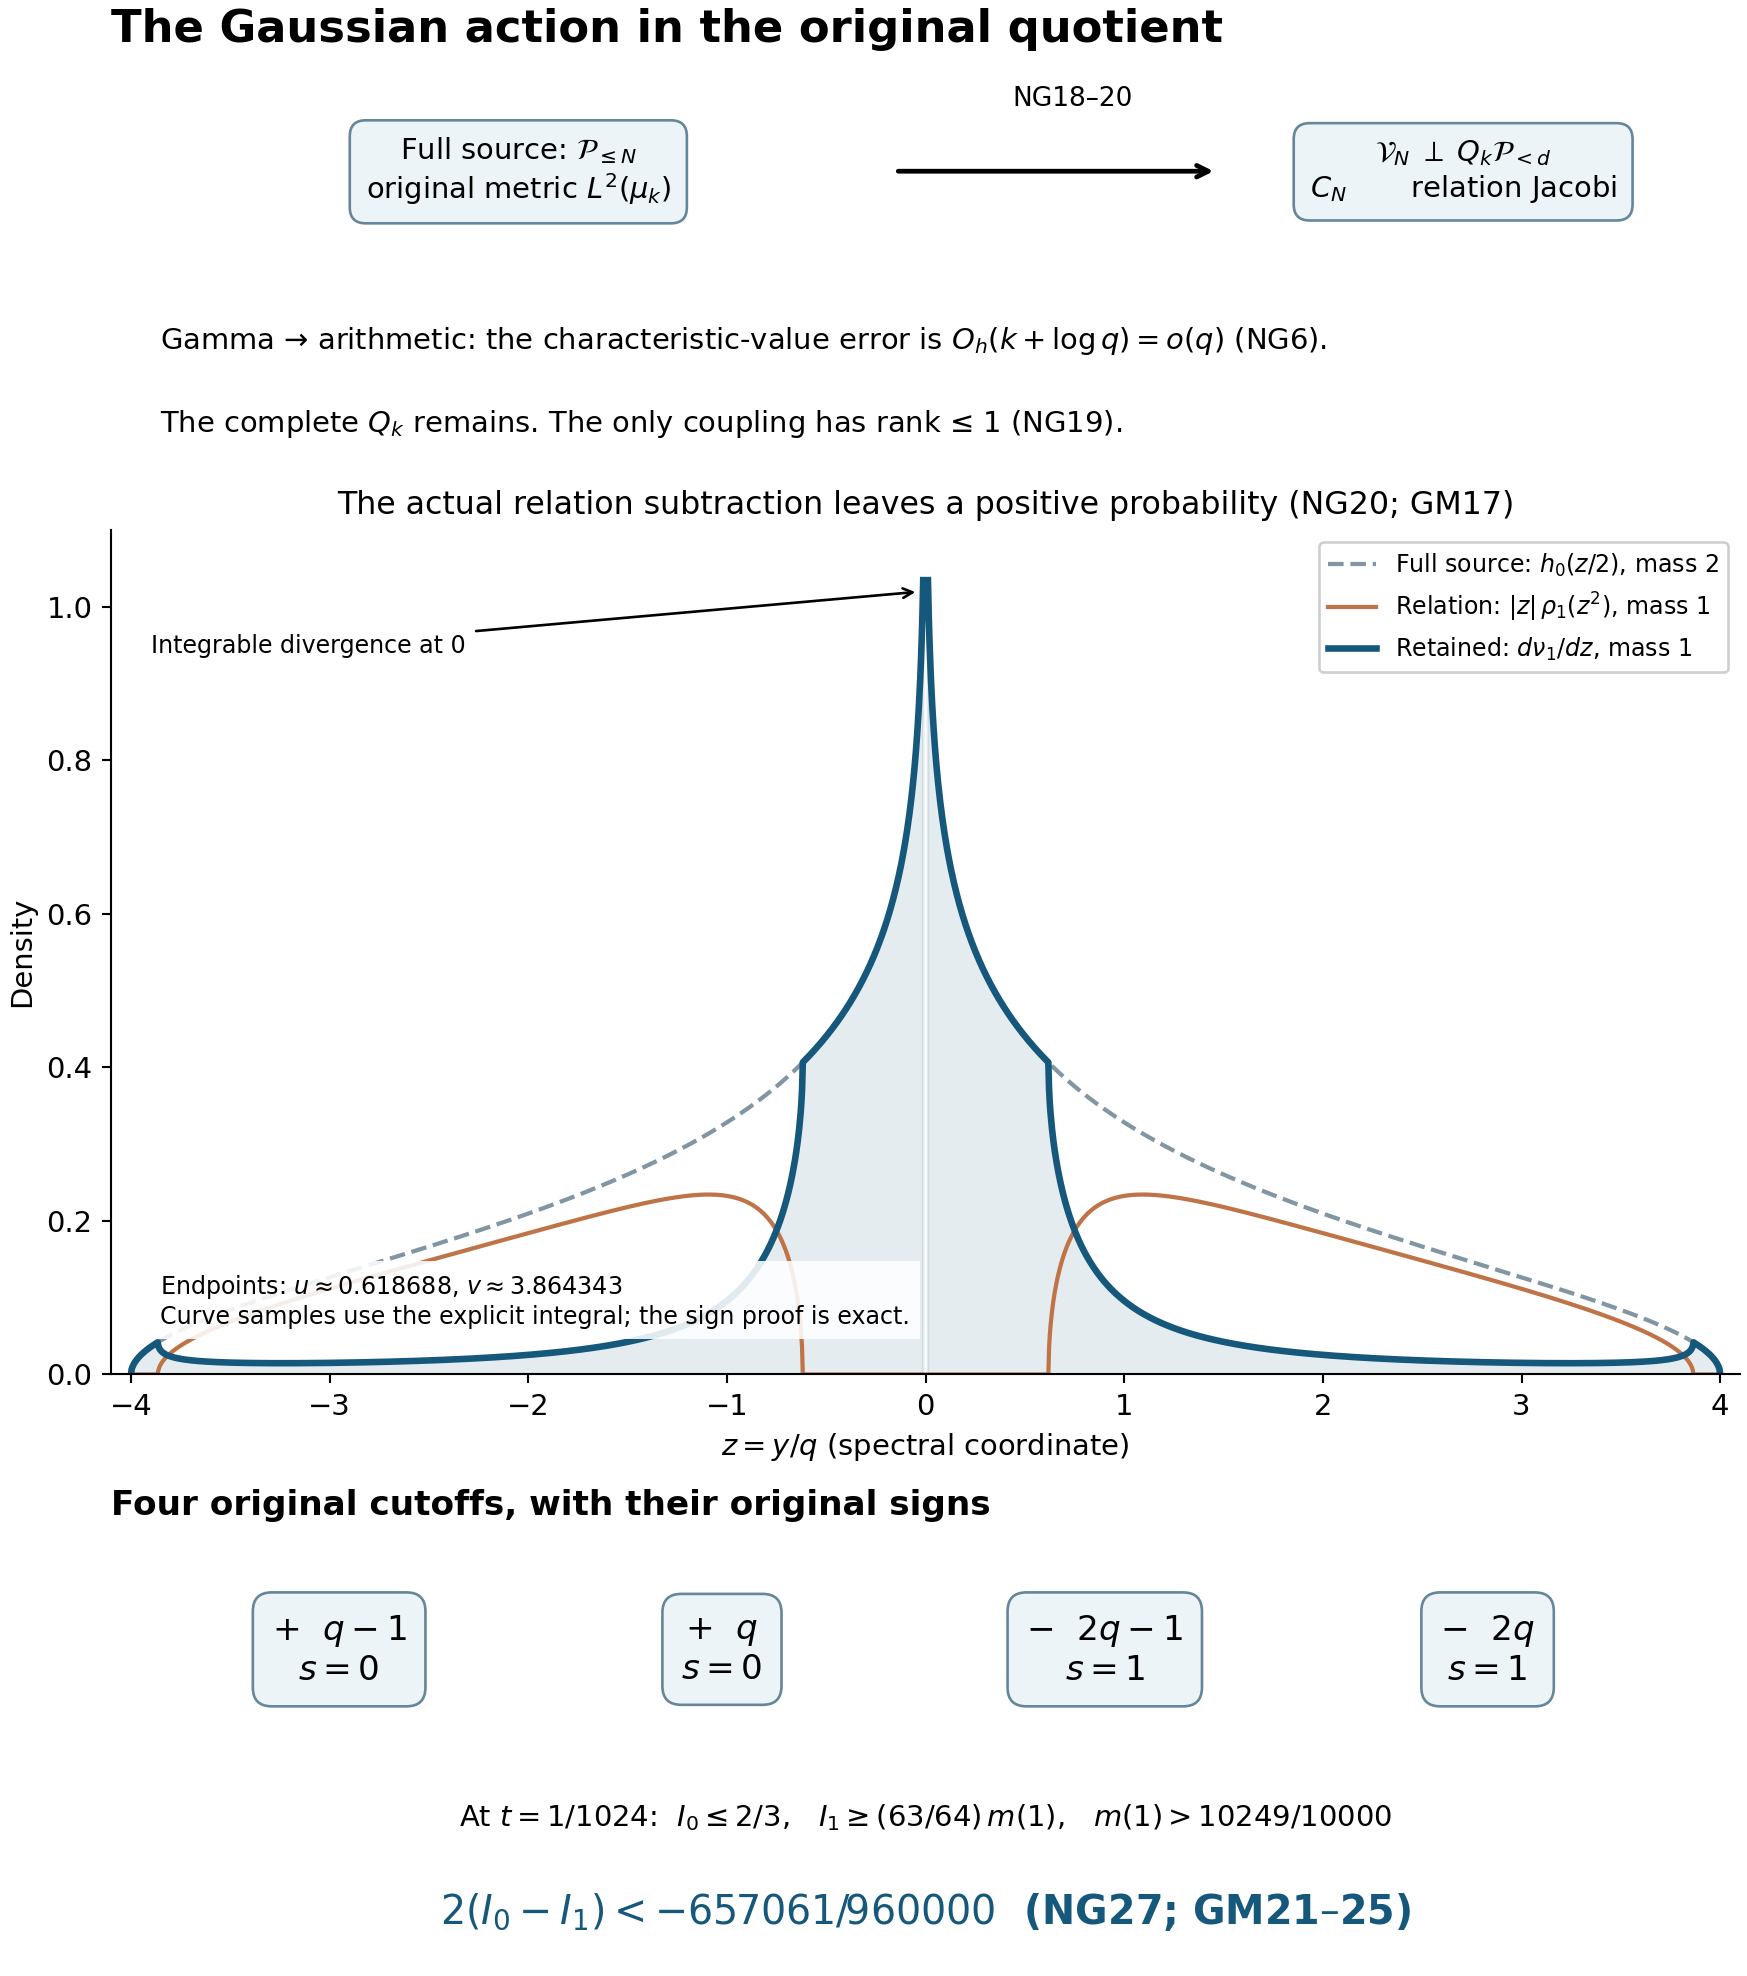
\includegraphics[width=\textwidth,height=.76\textheight,keepaspectratio]{GAUSSIAN_NATIVE_MECHANISM.png}
The complete original source and relation masses remain: at $s=1$,
$h_0(z/2)$ has mass two, $|z|\rho_1(z^2)$ has mass one, and their
difference is the positive probability density $d\nu_1/dz$.
The numerical curve samples illustrate NG10 and NG20; GM17 proves
positivity exactly. The origin has an integrable divergence.
The top panel is the actual source/relation splitting of NG18--20;
its coupling has rank at most one. The full polynomial $Q_k$ remains.
For the observation sign the domain is $m_0=1$, the proved five-orbit
domain $|u|\ge R_*$, and the original quotient metric (NG24).
In the lower panel $I_s=-H_s'(1/1024)$, distinct from the modified
Bessel function in NG25. The four original cutoffs and signs feed
NG27; GM21--25 give its explicit endpoint and rational bounds.
Human formula sources: Koornwinder et al., DLMF Chapter 18;
Forrester, arXiv:1806.10411v1, Sections 1--2.3, for Andr\'eief;
Carlson, DLMF Chapter 19, for elliptic conventions.
The complete proofs and point-of-use bibliography entries appear above.
\section*{How these calculations update the preceding arguments}
The original multiplication bound CAI16--25 now enters NG3--6.
NG12--15 uses the full root polynomial and the complete logarithmic
perturbation; NG20 then proves the original arithmetic compression
limit. NG23--27 carry this limit through the actual observation.
The orbit alternatives OQC10--13, OQX3 and MRI1d remain: the
five-member orbit, not the size-one orbit, supplies the small kernel.
The finite Weil form and SG9--17 remain different specified forms;
none is assigned a sign by the signed combination calculated here.
The seven absolute logarithmic allocations and individual projected
currents still require their own calculations. No RH conclusion or
effective finite-degree threshold is asserted.
\endgroup
% END COMPLETE ARITHMETIC GAUSSIAN RETURN 052

\end{document}
